\documentclass[a4paper,12pt]{extarticle}
\usepackage[utf8]{inputenc}
\usepackage[T1,T2A]{fontenc}
\usepackage[russian]{babel}
%% Отступы
\usepackage[left=2cm,right=2cm,top=2cm,bottom=2cm,bindingoffset=0cm]{geometry}
\usepackage{enumitem}

%% Картинки
\usepackage{graphicx} % для картинок
\graphicspath{{pic/}}
\usepackage{float} 

%% Точки нумерации заголовков
\usepackage{titlesec}
\titlelabel{\thetitle.\quad}
\usepackage[dotinlabels]{titletoc}

%% Нумерация картинок по секциям
\usepackage{chngcntr}
\counterwithin{figure}{section}
\counterwithin{table}{section}

%% Ставим шрифт Times New Roman
\usepackage{fontspec}
\setmainfont{Times New Roman}

%% Формат картинок
\usepackage{subcaption}
\DeclareCaptionLabelSeparator{custom}{ - }
\captionsetup {labelsep=custom}
\addto\captionsrussian{\renewcommand{\figurename}{Рис.}}
\usepackage[belowskip=2pt,aboveskip=2pt]{caption}
\setlength{\intextsep}{2pt plus 1pt minus 1pt}

%% Изменение отступов
\renewcommand{\baselinestretch}{1}
\setlength{\parskip}{0pt}
\setlength{\parindent}{1.15cm} % Отступ красной строки
\usepackage{titlesec}

% Настройка отступов для всех уровней заголовков
\titlespacing*{\section}{0pt}{0.5cm}{0.25cm}
\titlespacing*{\subsection}{0pt}{0.5cm}{0.25cm}
\titlespacing*{\subsubsection}{0pt}{0.5cm}{0.25cm}

%% Настройка шрифта заголовков
\titleformat{\section}{\normalfont\fontsize{16}{16}\selectfont\bfseries}{\thesection.}{1em}{}
\titleformat{\subsection}{\normalfont\fontsize{14}{14}\selectfont\bfseries}{\thesubsection.}{1em}{}
\titleformat{\subsubsection}{\normalfont\fontsize{13}{12}\selectfont\bfseries}{\thesubsubsection.}{1em}{}
\titleformat{\paragraph}{\normalfont\fontsize{13}{12}\selectfont\bfseries}{\theparagraph.}{1em}{}

%% Изменение оглавления
\usepackage{titletoc}
\titlecontents{section}[0.0cm]{}
{\thecontentslabel\enspace}{}
{{\titlerule*[1pc]{.}\contentspage}}
\titlecontents{subsection}[.4cm]{}
{\thecontentslabel\enspace}{}
{{\titlerule*[1pc]{.}\contentspage}}

\usepackage[unicode, colorlinks=true, linkcolor=black, citecolor=black, filecolor=black, urlcolor=black]{hyperref}

%% Выравнивание без переносов
\usepackage[none]{hyphenat}
\sloppy

%% Настройка нумерации
\usepackage{fancyhdr}
\pagestyle{fancy}
\fancyhf{}
\fancyfoot[R]{\thepage}
\renewcommand{\headrulewidth}{0pt}
\renewcommand{\footrulewidth}{0pt}
\pagenumbering{arabic}

%% Листинги
\usepackage{listings}
\usepackage{xcolor}

\definecolor{codegreen}{rgb}{0,0.6,0}
\definecolor{codegray}{rgb}{0.5,0.5,0.5}
\definecolor{codeblue}{rgb}{0.58,0,0.82}
\definecolor{backcolour}{rgb}{0.95,0.95,0.92}
\lstset{
    backgroundcolor=\color{backcolour},   
    commentstyle=\color{codegreen},
    keywordstyle=\color{blue},
    numberstyle=\tiny\color{codegray},
    stringstyle=\color{codeblue},
    basicstyle=\ttfamily\footnotesize,
    breakatwhitespace=false,         
    breaklines=true,                 
    captionpos=b,                    
    keepspaces=true,                 
    numbers=left,                    
    numbersep=5pt,                  
    showspaces=false,                
    showstringspaces=false,
    showtabs=false,                  
    tabsize=2
}

\begin{document}

\begingroup
\setlength{\parindent}{0cm} % временно отключаем отступ красной строки для титульной страницы
\begin{titlepage}	% начало титульной страницы

	\begin{center}		% выравнивание по центру

		\large Санкт-Петербургский политехнический университет Петра Великого\\[.4cm]
		\large Институт компьютерных наук и кибербезопастности \\[.4cm]
		\large Высшая школа компьютерных технологий и информационных систем\\[5cm]
		% название института, затем отступ 6см
		
		\Large \textbf{Отчёт по лабораторной оте №12}\\[0.3cm]
		\large Дисциплина: Телекоммуникационные технологии.\\[4cm]

	\end{center}

	\large Выполнил студент гр. 5130901/10101\hfill \underline{\hphantom{(12подпись12)}} \hfill М. Т. Непомнящий\\[.1cm]
	\large \hphantom{Выполнил студент гр. 5130901/10101}\hfill (подпись) \hfill \hphantom{М. Т. Непомнящий}\\[1.5cm]

	\large Руководитель \hphantom{дент гр. 513090}\hfill \underline{\hphantom{(12подпись12)}} \hfill Н.В. Богач\\[.1cm]
	\large \hphantom{Выполнил студент гр. 5130901/10101}\hfill (подпись) \hfill \hphantom{М. Т. Непомнящий}\\[2cm]

	\hfill\large \today

	\vfill % заполнить всё доступное ниже пространство

	\begin{center}
	\large Санкт-Петербург\\
	\large \the\year % вывести дату
	\end{center} % закончить выравнивание по центру

\end{titlepage} % конец титульной страницы

\vfill % заполнить всё доступное ниже пространство

\endgroup

\setlength{\parindent}{1.15cm} % включаем обратно отступ красной строки

\renewcommand\contentsname{\centerline{Содержание}}
\tableofcontents
\newpage

\section{Задача}\label{sec:s1}

\hspace{1.15cm}Исследовать применение FIR фильтра сдвига частоты в среде GNU Radio для 
понимания его функционала и эффективности в обработке сигналов. Основной 
задачей является изучение способов создания и настройки фильтровых коэффициентов 
(filter taps) для подавления высокочастотных помех и анализ влияния этих настроек 
на исходный сигнал. Дополнительной целью является оценка производительности фильтра 
при различных условиях работы, таких как изменение параметров фильтра и его частотного 
диапазона. Полученные результаты помогут глубже понять принципы работы FIR фильтров и 
их применимость в практических задачах обработки сигналов.

\section{Ход работы}

\subsection{Подготовка исходной схемы}\label{subsec:s2.1}

\subsubsection{Схема из 1 туториала}\label{subsec:s2.1.1}

\hspace{1.15cm}За основу для выполнения данного задания была взята схема, построенная в предыдущем 
задании (\href{https://wiki.gnuradio.org/index.php?title=Low_Pass_Filter_Example}
{Low Pass Filter Example}), где создавался простой фильтр низких частот в GNU Radio с 
использованием блоков "Variable", "QT GUI Range", "Signal Source" и "Low Pass Filter", 
"Throttle" и "QT GUI Frequency Sink".В конце задания создаётся графическая схема, которая 
генерирует сигнал, пропускает его через фильтр нижних частот и выводит результат на 
экран. Таким образом, была создана схема, представленная на Рис. \ref{fig:cos_schem} ниже:\\
\begin{figure}[H]
    \centering
    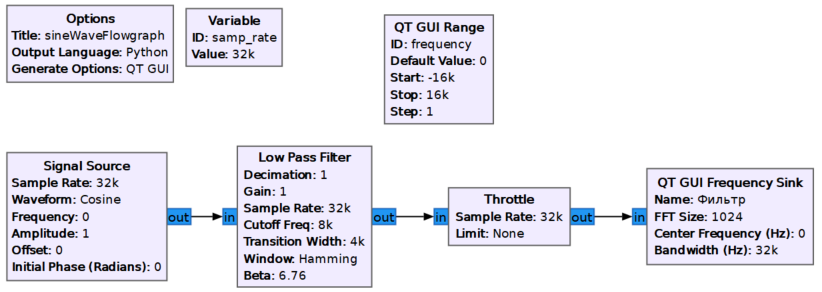
\includegraphics[width=.7\textwidth]{cos_schem}
    \caption{Схема из первого задания.} %% подпись к рисунку
    \label{fig:cos_schem} %% метка рисунка для ссылки на него
\end{figure}
Краткое описание блоков, используемых в схеме:
\begin{itemize}[nolistsep]
    \item \textbf{Varible} - используется для хранения переменной \textit{samp\_rate,} 
    от которой будут отсчитываться остальные частоты в проекте.
    \item \textbf{QT GUI Range} - используется для изменения значения частоты сигнала
    в процессе моделирования.
    \item \textbf{Signal Source} - генератор косинусоидальный сигнала с частотой, подаваемой
    с QT GUI Range и амплитудой 1.
    \item \textbf{Low Pass Filter} - исследуемый фильтр низких частот, он имеет несколько параметров, 
    которые будут рассмотрены позднее. 
    \item \textbf{Throttle} - предназначенный для ограничения скорости передачи сэмплов в цифровой 
    обработке сигналов. Проще говоря ограничитель скорости передачи данных. 
    \item \textbf{QT GUI Frequency Sink} - это графический приемник, основанный на библиотеке QT, 
    предназначенный для отображения нескольких сигналов в частотной области.
\end{itemize}
\vspace{0.5cm}

\newpage
\subsubsection{Low Pass Filter}

\hspace{1.15cm}Одним из ключивых элементов схемы является \textbf{Low Pass Filter}, рассмотрим его отдельно:\\
\begin{figure}[H]
    \centering
    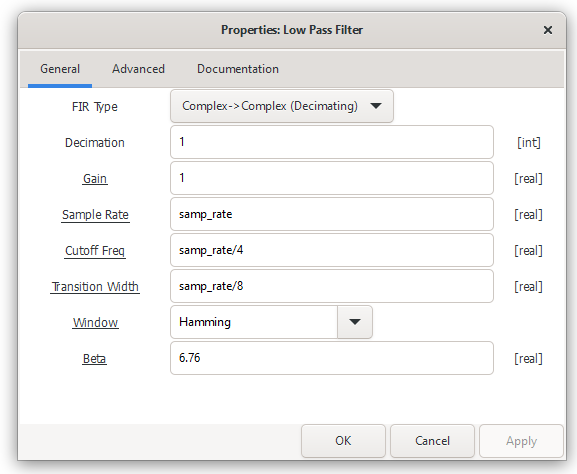
\includegraphics[width=.5\textwidth]{Low_Pass}
    \caption{Настройки Low Pass Filter.} %% подпись к рисунку
    \label{fig:Low_Pass} %% метка рисунка для ссылки на него
\end{figure}
Разберём за что отвечает каждый из параметров:
\vspace{0.25cm}
\begin{itemize}[nolistsep]
    \item \textbf{FIR Type} - определяет тип FIR фильтра, то есть указывает, работает ли 
    фильтр с вещественными или комплексными входными/выходными данными.
    \item \textbf{Decimation} - определяет коэффициент децимации фильтра, который указывает, 
    на сколько раз уменьшается частота дискретизации сигнала после применения фильтра.
    \item \textbf{Gain} - масштабирующий коэффициент, применяемый к выходу фильтра, 
    для регулировки амплитуды сигнала.
    \item \textbf{Sample Rate} - частота дискретизации входного сигнала, указывает, с 
    какой частотой входные сигналы отсчитываются во времени. 
    \item \textbf{Cutoff Freq} - частота среза фильтра, то есть частота, на 
    которой фильтр начинает подавлять высокочастотные составляющие входного сигнала.
    \item \textbf{Transition Width} - ширина переходной зоны между полосой подавления 
    и полосой пропускания в фильтре. Этот параметр указывает, насколько широкой 
    должна быть зона плавного перехода между частотами, на которых фильтр полностью 
    подавляет или пропускает сигнал.
    \item \textbf{Window} - тип окна, используемого при генерации коэффициентов фильтра. 
    Различные типы окон имеют разные свойства и влияют на характеристики фильтра, такие 
    как разрешение в частотной области и уровень подавления сигнала.
    \item \textbf{Beta} - параметр, который применяется только к окну Кайзера. 
    Этот параметр контролирует форму окна Кайзера и влияет на его способность 
    сглаживания переходной зоны и подавления побочных лепестков.
\end{itemize}
\vspace{0.25cm}
\hspace{1.15cm}Таким образом, мы создали схему (Рис. \ref{fig:cos_schem}) 
из первого туториала и готовы перейти к основной части проекта (\href
{https://wiki.gnuradio.org/index.php?title=Designing_Filter_Taps}{Designing Filter Taps}).

\newpage
\subsection{Designing the Filter Taps}

\subsubsection{Frequency Xlating FIR Filter}

\hspace{1.15cm}Немного изменим схему, заменив фильтр нижних частот (\textbf{Low Pass Filter}) на цифровой FIR-фильтр 
с возможностью сдвига частоты (\textbf{Frequency Xlating FIR Filter}). Его настройки представлены на Рис. 
\ref{fig:FIR_Filter} ниже:\\
\begin{figure}[H]
    \centering
    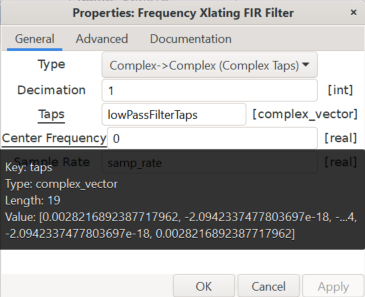
\includegraphics[width=.7\textwidth]{FIR_Filter}
    \caption{Настройки Frequency Xlating FIR Filter.} %% подпись к рисунку
    \label{fig:FIR_Filter} %% метка рисунка для ссылки на него
\end{figure}
Разберём за что отвечает каждый из его параметров:
\vspace{0.15cm}

\begin{itemize}
    
    \item \textbf{Type (Тип фильтра)}
    \begin{itemize}
        \item \textit{Описание}: Указывает тип фильтра, который будет применен к сигналу.
        \item \textit{Примеры}: Низкочастотный фильтр (Lowpass Filter), Высокочастотный фильтр (Highpass Filter), Полосовой фильтр (Bandpass Filter), Режекторный фильтр (Bandstop Filter), Произвольный тип фильтра, определенный пользователем.
    \end{itemize}

    \item \textbf{Decimation (Децимация)}
    \begin{itemize}
        \item \textit{Описание}: Указывает коэффициент децимации, который определяет, насколько уменьшится частота дискретизации после фильтрации. Децимация снижает частоту дискретизации сигнала, оставляя только каждую n-ю выборку.
        \item \textit{Пример}: Если указано значение 4, выходная частота дискретизации будет в 4 раза меньше входной.
    \end{itemize}

    \item \textbf{Taps (Коэффициенты фильтра)}
    \begin{itemize}
        \item \textit{Описание}: Это список коэффициентов FIR-фильтра. Эти коэффициенты определяют характеристики фильтра, такие как полоса пропускания и крутизна спада. Коэффициенты могут быть рассчитаны с использованием различных методов проектирования фильтров, таких как окно Хэмминга, окно Кайзера и другие.
        \item \textit{Пример}: \texttt{[0.1, 0.15, 0.5, 0.15, 0.1]} - пример простого набора коэффициентов.
    \end{itemize}

    \item \textbf{Center Frequency (Центральная частота)}
    \begin{itemize}
        \item \textit{Описание}: Определяет частоту, на которую необходимо сместить входной сигнал. Это значение указывает, на сколько герц сигнал будет сдвинут вверх или вниз по частоте.
        \item \textit{Пример}: Если указать значение 100 kHz, входной сигнал будет смещен на 100 kHz вверх по частоте.
    \end{itemize}

    \item \textbf{Sample Rate (Частота дискретизации)}
    \begin{itemize}
        \item \textit{Описание}: Указывает частоту дискретизации входного сигнала. Этот параметр необходим для правильной настройки частоты и фильтрации.
        \item \textit{Пример}: Если входная частота дискретизации равна 1 MHz, это значение нужно указать в соответствующем параметре.
    \end{itemize}
\end{itemize}
\vspace{0.25cm}

Данный фильтр используется для изменения частоты сигнала путем умножения на комплексный синус 
или косинус. Этот процесс позволяет сдвигать спектр сигнала в частотной области, что полезно 
для различных задач обработки сигналов, таких как смещение частоты сигнала для согласования с 
другими устройствами или для избегания помех. Суть элемента Frequency Xlating FIR Filter 
заключается в его способности выполнять эффективное цифровое смещение частоты в потоке данных 
сигнала.
\vspace{0.25cm}\\
\vspace{0.25cm}
\textbf{*Пояснение}

Умножение сигнала на комплексный синус или косинус используемая для сдвига частоты сигнала в 
цифровой обработке сигналов. Комплексный синус или косинус представляется в виде 
\(e^{j\omega t} = \cos(\omega t) + j\sin(\omega t)\), где \(\omega\) — угловая частота, \(t\) — 
время, а \(j\) — мнимая единица.
\vspace{0.25cm}\\
\textbf{Как это работает}

\begin{enumerate}
    \item \textbf{Исходный сигнал}: Пусть \(s(t)\) — это наш исходный сигнал с некоторой спектральной составляющей.
    \item \textbf{Комплексный синус или косинус}: Для сдвига частоты мы умножаем \(s(t)\) на \(e^{j\omega t}\):
    \[
    s(t) \cdot e^{j\omega t}
    \]
    \item \textbf{Результат умножения}: В результате умножения сигнала на \(e^{j\omega t}\) происходит сдвиг всех частотных составляющих сигнала на \(\omega\) в частотной области. Это можно объяснить с помощью свойства преобразования Фурье:
    \[
    \mathcal{F}\{s(t) \cdot e^{j\omega t}\} = S(f - \frac{\omega}{2\pi})
    \]
    где \(S(f)\) — спектр исходного сигнала, а \(f\) — частота. Таким образом, весь спектр сигнала \(s(t)\) сдвигается на \(\frac{\omega}{2\pi}\).
\end{enumerate}


\newpage
\subsubsection{Low-Pass Filter Taps}

\hspace{1.15cm}Также добавим на схему элемент Low-Pass Filter Taps, выставиви следующие настройки:\\
\begin{figure}[H]
    \centering
    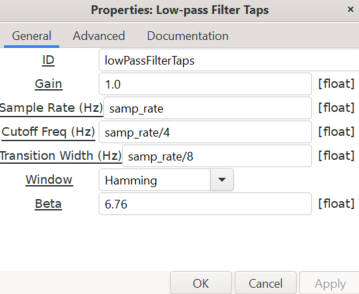
\includegraphics[width=.7\textwidth]{Low_Pass_Taps}
    \caption{Исходная схема.} %% подпись к рисунку
    \label{fig:Low_Pass_Taps} %% метка рисунка для ссылки на него
\end{figure}

Элемент \textbf{Low-Pass Filter Taps} в GNU Radio используется для создания набора коэффициентов 
для низкочастотного фильтра (FIR-фильтра). Эти коэффициенты затем могут быть использованы в 
различных блоках для фильтрации сигнала. Вот основные параметры этого блока и их описание:

\begin{itemize}
    \item \textbf{Sample Rate (Частота дискретизации)}
    \begin{itemize}
        \item \textit{Описание}: Указывает частоту дискретизации входного сигнала, на основе которой будет рассчитан фильтр.
        \item \textit{Пример}: Если входная частота дискретизации равна 1 MHz, это значение нужно указать в соответствующем параметре.
    \end{itemize}

    \item \textbf{Cutoff Frequency (Частота среза)}
    \begin{itemize}
        \item \textit{Описание}: Определяет частоту, выше которой сигнал будет подавляться. Это ключевой параметр, который определяет границу полосы пропускания фильтра.
        \item \textit{Пример}: Если указано значение 100 kHz, то частоты выше 100 kHz будут подавляться.
    \end{itemize}

    \item \textbf{Transition Width (Ширина переходной области)}
    \begin{itemize}
        \item \textit{Описание}: Определяет ширину полосы частот, в которой фильтр переходит от пропускания к подавлению. Ширина переходной области влияет на крутизну отклика фильтра.
        \item \textit{Пример}: Если указана ширина 10 kHz, фильтр будет переходить от полного пропускания частот ниже частоты среза к полному подавлению частот выше частоты среза в диапазоне 10 kHz.
    \end{itemize}

    \item \textbf{Window}
    \begin{itemize}
        \item \textit{Описание}: Определяет тип оконной функции, используемой для расчета коэффициентов фильтра. Различные оконные функции имеют разные характеристики и влияют на форму отклика фильтра.
        \item \textit{Примеры}:
        \begin{itemize}
            \item \texttt{Hamming} (Хэмминг)
            \item \texttt{Hann} (Ханн)
            \item \texttt{Blackman} (Блэкман)
            \item \texttt{Kaiser} (Кайзер)
        \end{itemize}
    \end{itemize}

    \item \textbf{Beta}
    \begin{itemize}
        \item \textit{Описание}: Параметр окна Кайзера. Используется только если выбрано окно Кайзера. Этот параметр определяет форму окна Кайзера и контролирует компромисс между шириной главного лепестка и уровнем боковых лепестков.
        \item \textit{Пример}: Типичное значение для бета может быть 8.6.
    \end{itemize}
\end{itemize}
\hspace{1.15cm}Эти параметры позволяют точно настраивать характеристики низкочастотного фильтра для решения задач фильтрации сигнала в реальном времени.

\vspace{0.25cm}После всех описанных ранее действий мы получим следующую схему:\\
\begin{figure}[H]
    \centering
    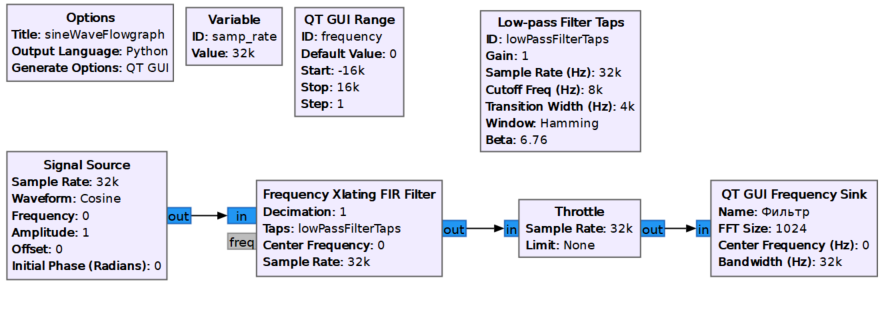
\includegraphics[width=.7\textwidth]{schem_1}
    \caption{Схема Designing the Filter Taps.} %% подпись к рисунку
    \label{fig:schem_1} %% метка рисунка для ссылки на него
\end{figure}

Таким образом, мы создали схему с частотно-смещающим фильтром с возможностью настройки
частоты и визуализации спектра сигнала в реальном времени.

\subsubsection{Анализ схемы}

Рассмотрим полученную выше схему (Рис. \ref{fig:schem_1}) подробнее.

\paragraph{Принцип работы}

\begin{enumerate}
    \item \textbf{Signal Source (Источник сигнала)}: Генерирует косинусоидальный сигнал с частотой 0 Гц (постоянный сигнал) с амплитудой 1 и частотой дискретизации 32 кГц.
    \item \textbf{QT GUI Range (Диапазон частот для GUI)}: Позволяет пользователю изменять частоту сигнала от -16 кГц до 16 кГц в шаге 1 Гц с помощью графического интерфейса.
    \item \textbf{Low-Pass Filter Taps (Коэффициенты фильтра нижних частот)}: Определяет параметры фильтра нижних частот с частотой дискретизации 32 кГц, частотой среза 8 кГц и шириной перехода 4 кГц с использованием окна Хэмминга.
    \item \textbf{Frequency Xlating FIR Filter (Частотно-смещающий FIR фильтр)}: Применяет низкочастотный фильтр к входному сигналу, а также позволяет смещать частоту сигнала. Центр частоты и дискретизации фильтра соответствуют входным параметрам.
    \item \textbf{Throttle (Регулятор скорости)}: Ограничивает скорость потока данных, чтобы соответствовать реальному времени. Здесь нет ограничений по скорости.
    \item \textbf{QT GUI Frequency Sink (График частоты)}: Отображает спектр сигнала на графике. Параметры: размер FFT 1024, центральная частота 0 Гц, полоса пропускания 32 кГц.
\end{enumerate}

\paragraph{Предположения о поведении сигнала}
\begin{itemize}

    \item \textbf{От -16 до -8 кГц и от 8 до 16 кГц:}
    \begin{itemize}
        \item В этих диапазонах выходной сигнал будет подавлен до почти нулевого уровня, так как фильтр нижних частот срежет компоненты сигнала выше 8 кГц.
    \end{itemize}

    \item \textbf{От -8 до 8 кГц:}
    \begin{itemize}
        \item В этом диапазоне частот сигнал будет проходить через фильтр. Сигналы ближе к 0 Гц (DC) будут проходить без значительного ослабления.
        \item По мере приближения к частотам 8 кГц или -8 кГц, амплитуда сигнала начнет уменьшаться из-за переходной ширины фильтра (4 кГц).
    \end{itemize}

\end{itemize}

\paragraph{Пояснения}
\begin{itemize}

    \item \textbf{Низкочастотный фильтр:}
    \begin{itemize}
        \item Пропускает частоты ниже 8 кГц, а частоты выше 8 кГц ослабляет.
        \item Переходная ширина 4 кГц означает, что ослабление будет происходить постепенно в диапазоне от 8 кГц до 12 кГц.
    \end{itemize}

    \item \textbf{Frequency Xlating FIR Filter:}
    \begin{itemize}
        \item Перемещает центральную частоту сигнала на заданное значение, что позволяет нам наблюдать изменение частоты в широком диапазоне.
    \end{itemize}

    \item \textbf{QT GUI Frequency Sink:}
    \begin{itemize}
        \item Позволяет визуально наблюдать спектр сигнала и подтверждать теоретические расчеты и предположения о работе фильтра и изменения частоты.
    \end{itemize}

\end{itemize}

\subsubsection{Запуск блок-схемы}
\hspace{1.15cm}Проверим наши предположения, выполнив запуск схемы, представленной на Рис. 
\ref{fig:schem_1}. Установим настройку \textit{Max Hold} (Максимальное удержание). 
Когда эта опция включена, график показывает максимальное значение сигнала, которое было 
достигнуто в течение заданного времени, а затем удерживает его на экране. В результате получим 
график Частотного спектра выходного сигнала после применения частотно-смещающего фильтра:\\
\begin{figure}[H]
    \centering
    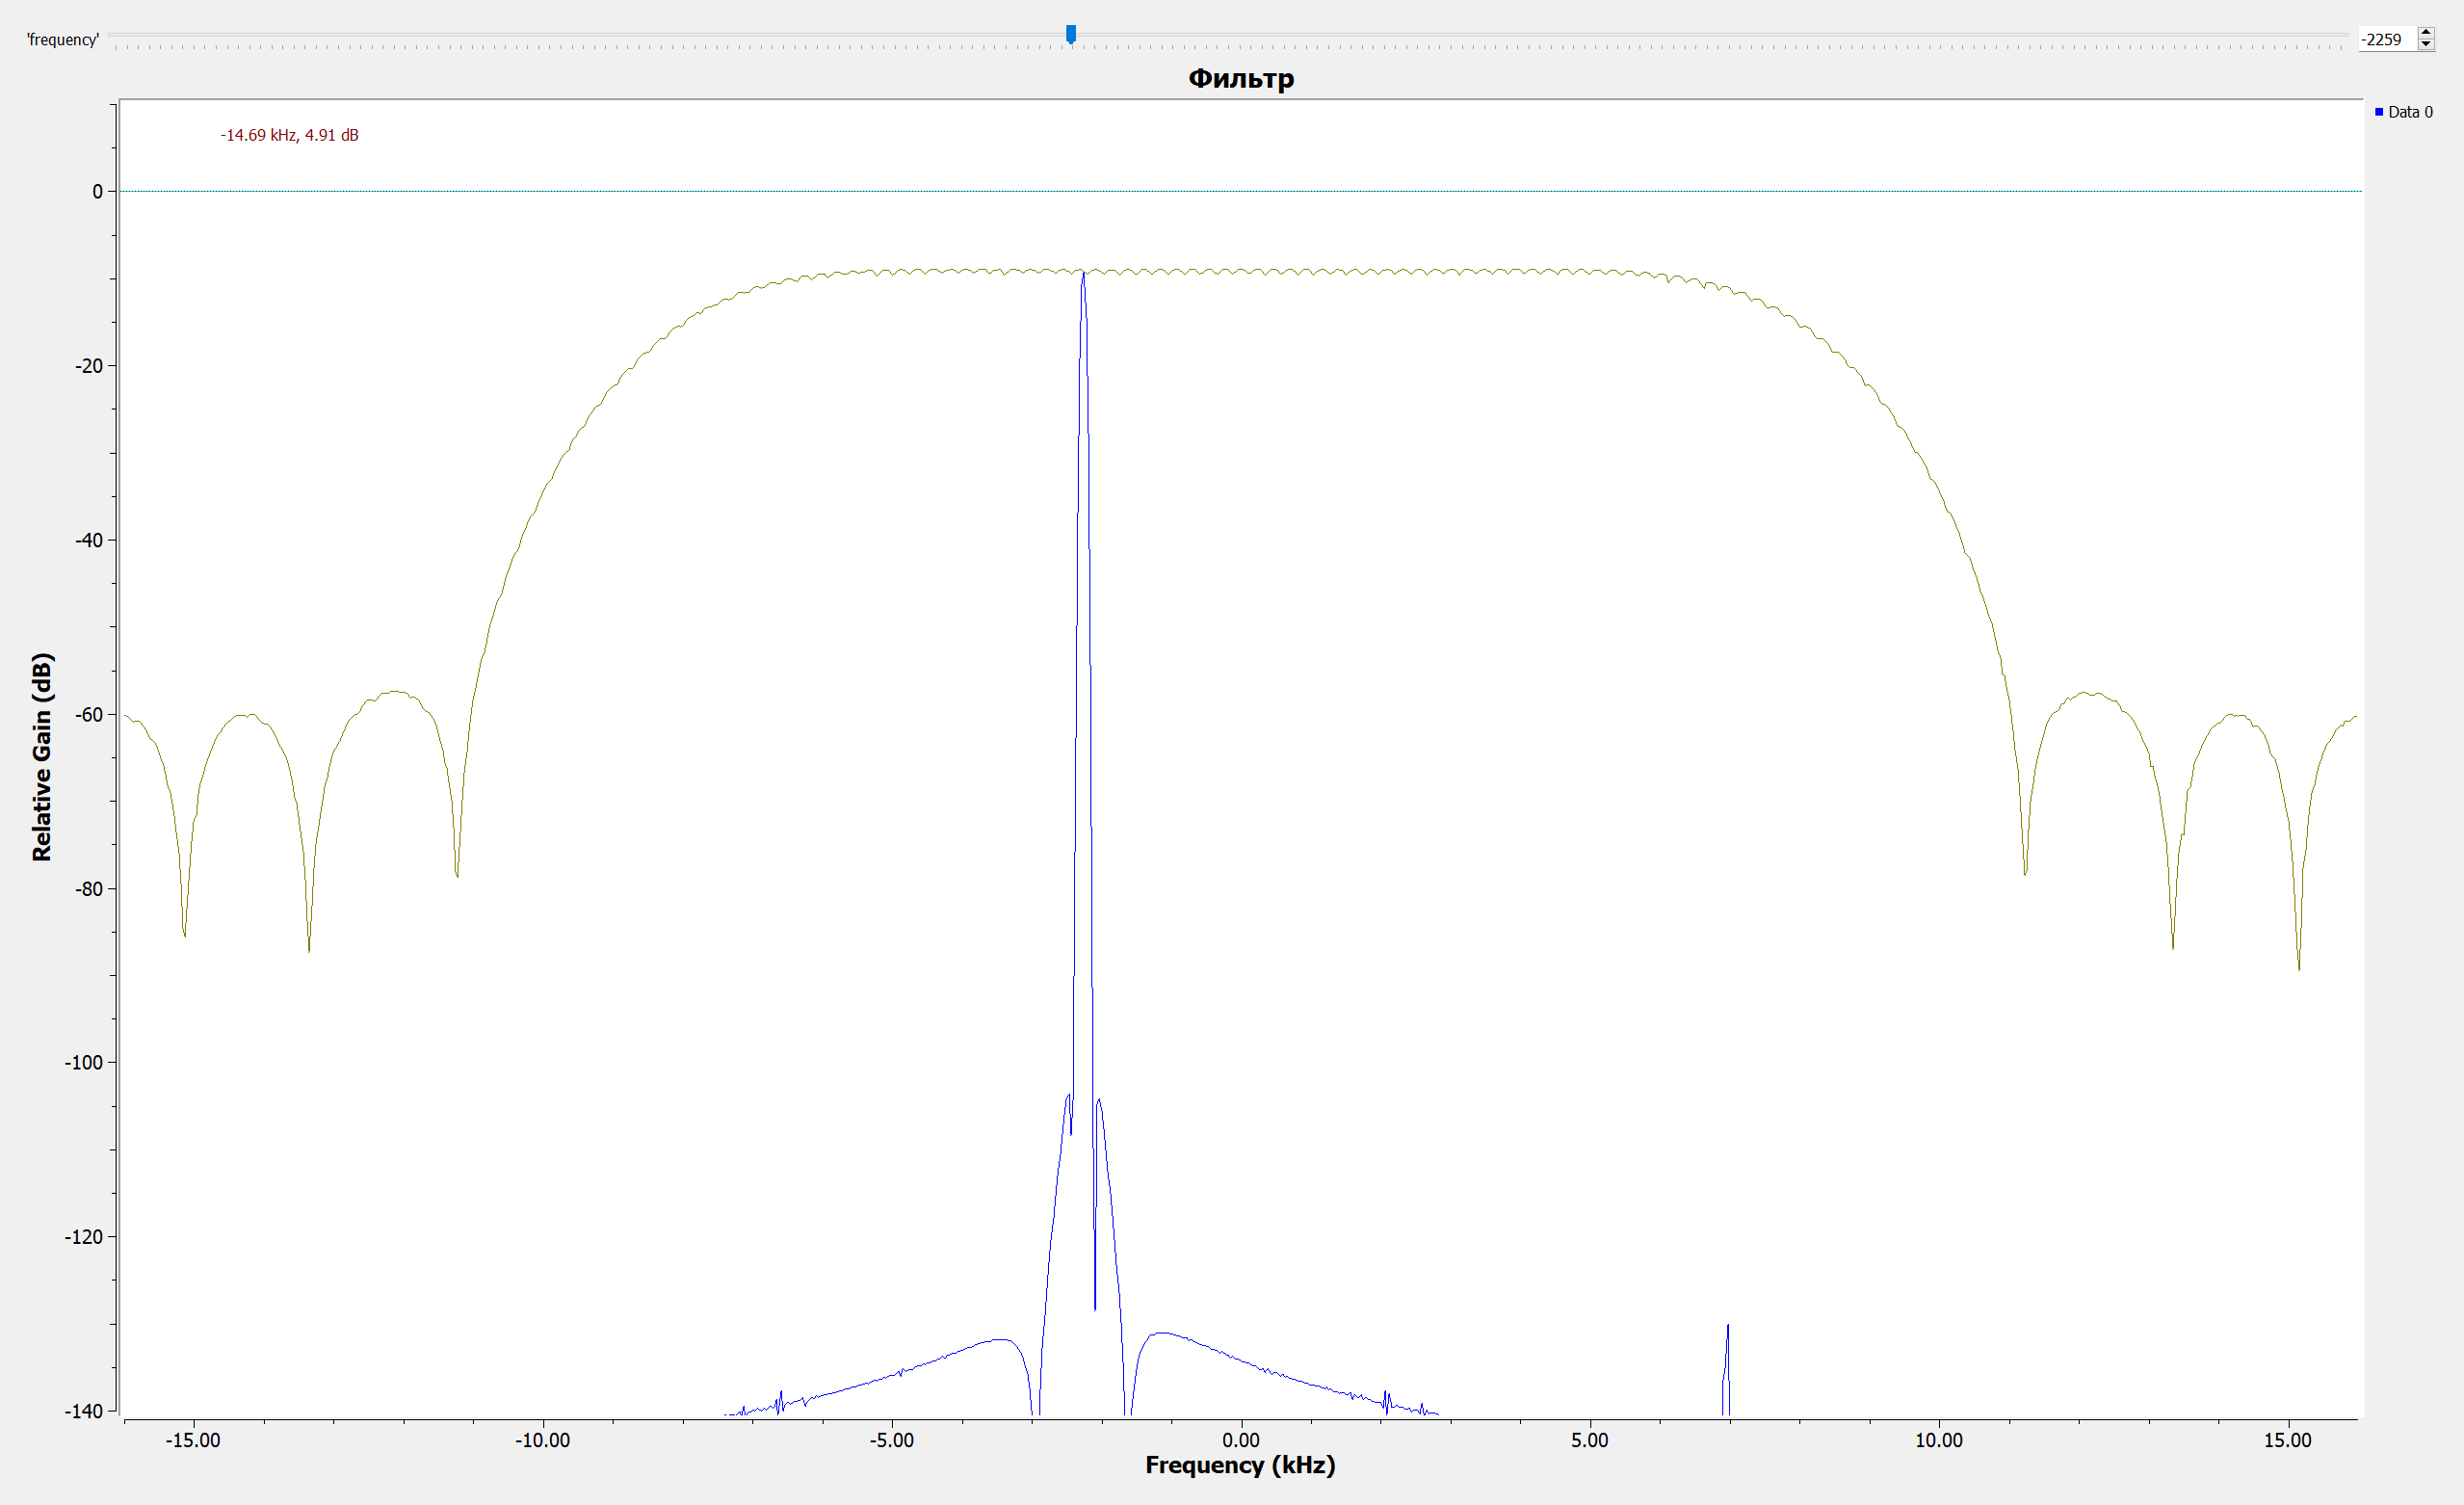
\includegraphics[width=.7\textwidth]{graph_1}
    \caption{График максимальных значений сигнала для 1 схемы.} %% подпись к рисунку
    \label{fig:graph_1} %% метка рисунка для ссылки на него
\end{figure}

\subsubsection{Анализ графика}

\hspace{1.15cm}График соответствует ожиданиям и отражает работу частотно-смещающего фильтра и влияния фильтра 
нижних частот. Рассмотрим основные особенности графика:

\begin{itemize}
    \item \textbf{Центральный пик на 0 Гц:}
    \begin{itemize}
        \item График показывает выраженный пик на 0 Гц, который соответствует исходному сигналу с частотой 0 Гц. Это то, что ожидалось, так как первоначально генерируемый сигнал имеет частоту 0 Гц (DC-компонента).
    \end{itemize}
    
    \item \textbf{Распределение частотного диапазона:}
    \begin{itemize}
        \item Частотный диапазон от -16 кГц до 16 кГц на графике совпадает с диапазоном изменения частоты в QT GUI Range.
    \end{itemize}
    
    \item \textbf{Фильтрация сигнала:}
    \begin{itemize}
        \item График показывает, что сигнал в пределах полосы пропускания фильтра (от -8 кГц до 8 кГц) остается неизменным или минимально ослабленным.
        \item За пределами полосы пропускания фильтра (выше 8 кГц и ниже -8 кГц) сигнал значительно ослаблен, что соответствует характеристикам фильтра нижних частот с частотой среза 8 кГц и шириной перехода 4 кГц.
    \end{itemize}
    
    \item \textbf{Переходная область фильтра:}
    \begin{itemize}
        \item Наблюдаются плавные переходы на частотах близких к 8 кГц и -8 кГц. Это соответствует переходной области фильтра, где амплитуда сигнала постепенно уменьшается.
    \end{itemize}
    
\end{itemize}

\paragraph{Соответствие ожиданиям:}
\begin{itemize}
    \item График подтверждает правильную работу частотно-смещающего FIR фильтра и его соответствие теоретическим ожиданиям.
    \item Фильтр нижних частот эффективно ослабляет компоненты сигнала выше 8 кГц и ниже -8 кГц, что подтверждается наблюдаемыми минимумами в этих областях.
    \item Частотно-смещающий механизм работает корректно, поскольку при изменении частоты ползунком спектр смещается, но при этом фильтрация сохраняет свою эффективность.
\end{itemize}

В общем, график соответствует ожиданиям и наглядно демонстрирует, как работает фильтр и как 
частота сигнала изменяется в рассматриваемом диапазоне.

\subsection{Entering Filter Taps Manually}

\hspace{1.15cm}В данном разделе мы рассмотрим использование блока Frequency \textbf{Xlating FIR Filter} с вручную 
введенными коэффициентами фильтра (filter taps) для обработки сигналов в GNU Radio.

\subsubsection{Изменение схемы}

\begin{itemize}
    \item Альтернативные методы можно использовать для проектирования отводов фильтра, а затем ввести 
    их вручную в качестве переменной Python. Например, блок Frequency \textbf{Xlating FIR Filter} 
    принимает отводы фильтра в виде массива NumPy. Чтобы иметь доступ к функциям и типам данных 
    NumPy, его необходимо сначала импортировать. Для этого добавим блок \textbf{Import} в рабочую 
    область GRC и в качестве начтройки Import введём \texttt{import numpy as np}.
    \item Простой фильтр скользящей средней, или \texttt{boxcar}, можно спроектировать, установив 
    все фильтрующие краны одинаковыми. Это можно сделать с помощью функции \texttt{NumPy ones()}, 
    которая возвращает массив NumPy всех единиц с указанной длиной. Создадим переменную с именем 
    boxcarFilter со значением \texttt{np.ones(8)/8}.
    \item Временно отключим блок \textbf{Low-Pass Filter Taps}, а в окне настройки блока 
    \textbf{Frequency Xlating FIR Filter} в строке Taps укажем \texttt{boxcarFilter}
\end{itemize}

\vspace{0.25cm}После всех описанных ранее действий мы получим следующую схему:\\
\begin{figure}[H]
    \centering
    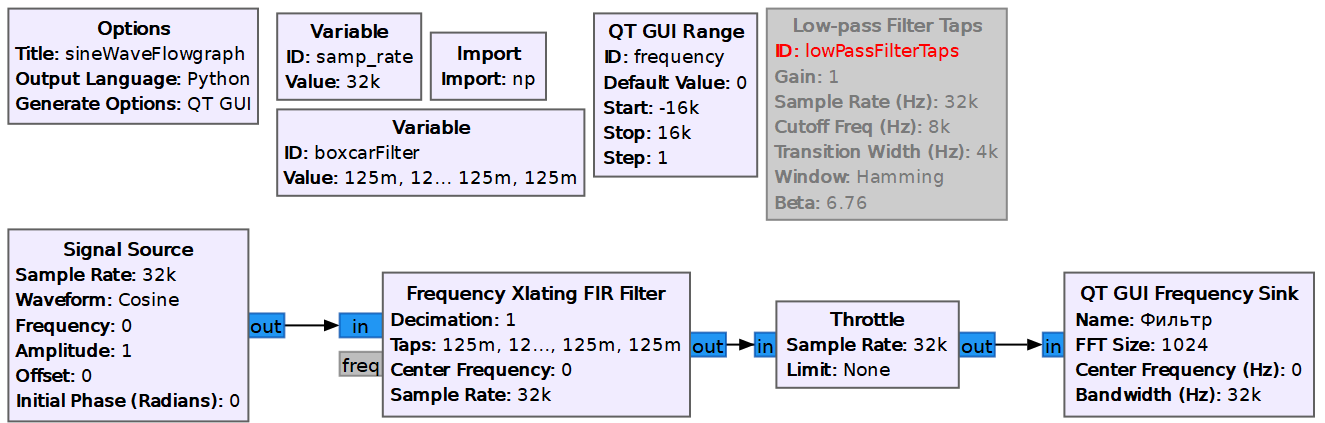
\includegraphics[width=.7\textwidth]{schem_2}
    \caption{Схема Entering Filter Taps Manually.} %% подпись к рисунку
    \label{fig:schem_2} %% метка рисунка для ссылки на него
\end{figure}

\subsubsection{Анализ схемы}

Рассмотрим полученную выше схему (Рис. \ref{fig:schem_2}) подробнее.

\paragraph{Принцип работы}

\begin{enumerate}
    \item \textbf{Блоки схемы:}
    \begin{itemize}
        \item \textbf{Signal Source}: Ггенерирует входной сигнал.
        \item \textbf{Frequency Xlating FIR Filter}: осуществляет фильтрацию сигнала, используя заданные вручную коэффициенты фильтра.
        \item \textbf{Sink (например, Time Sink и Frequency Sink)}: визуализируют обработанный сигнал в временной и частотной областях.
    \end{itemize}
    \item \textbf{Коэффициенты фильтра:}
    \begin{itemize}
        \item Коэффициенты фильтра задаются вручную в виде массива значений, 
        которые определяют характеристики фильтра, такие как полоса пропускания и 
        затухание за ее пределами.
    \end{itemize}
\end{enumerate}

\paragraph{Предположения о поведении сигнала}
\begin{itemize}

    \item \textbf{Центр полосы пропускания (0 кГц):}
    \begin{itemize}
        \item Сигнал на частотах, близких к 0 кГц, будет практически полностью проходить через фильтр.
    \end{itemize}

    \item \textbf{Границы полосы пропускания (-8 кГц и 8 кГц):}
    \begin{itemize}
        \item Здесь можно ожидать небольшое ослабление сигнала, так как границы фильтра обычно имеют постепенный переход.
    \end{itemize}

    \item \textbf{За пределами полосы пропускания (-16 кГц и 16 кГц):}
    \begin{itemize}
        \item Эти частоты будут значительно подавлены. Сигнал здесь будет почти полностью удален, особенно если фильтр имеет крутые переходы.
    \end{itemize}

\end{itemize}

Выходной сигнал будет изменяться в зависимости от частотного содержания входного сигнала и 
характеристик заданного фильтра. В пределах полосы пропускания сигнал будет проходить с 
минимальными изменениями, в то время как частоты за ее пределами будут подавлены.

\subsubsection{Запуск блок-схемы}
\hspace{1.15cm}Проверим наши предположения, выполнив запуск схемы, представленной на Рис. 
\ref{fig:schem_2}. Установим настройку \textit{Max Hold} (Максимальное удержание). 
Когда эта опция включена, график показывает максимальное значение сигнала, которое было 
достигнуто в течение заданного времени, а затем удерживает его на экране. В результате получим 
график Частотного спектра выходного сигнала после применения частотно-смещающего фильтра:\\
\begin{figure}[H]
    \centering
    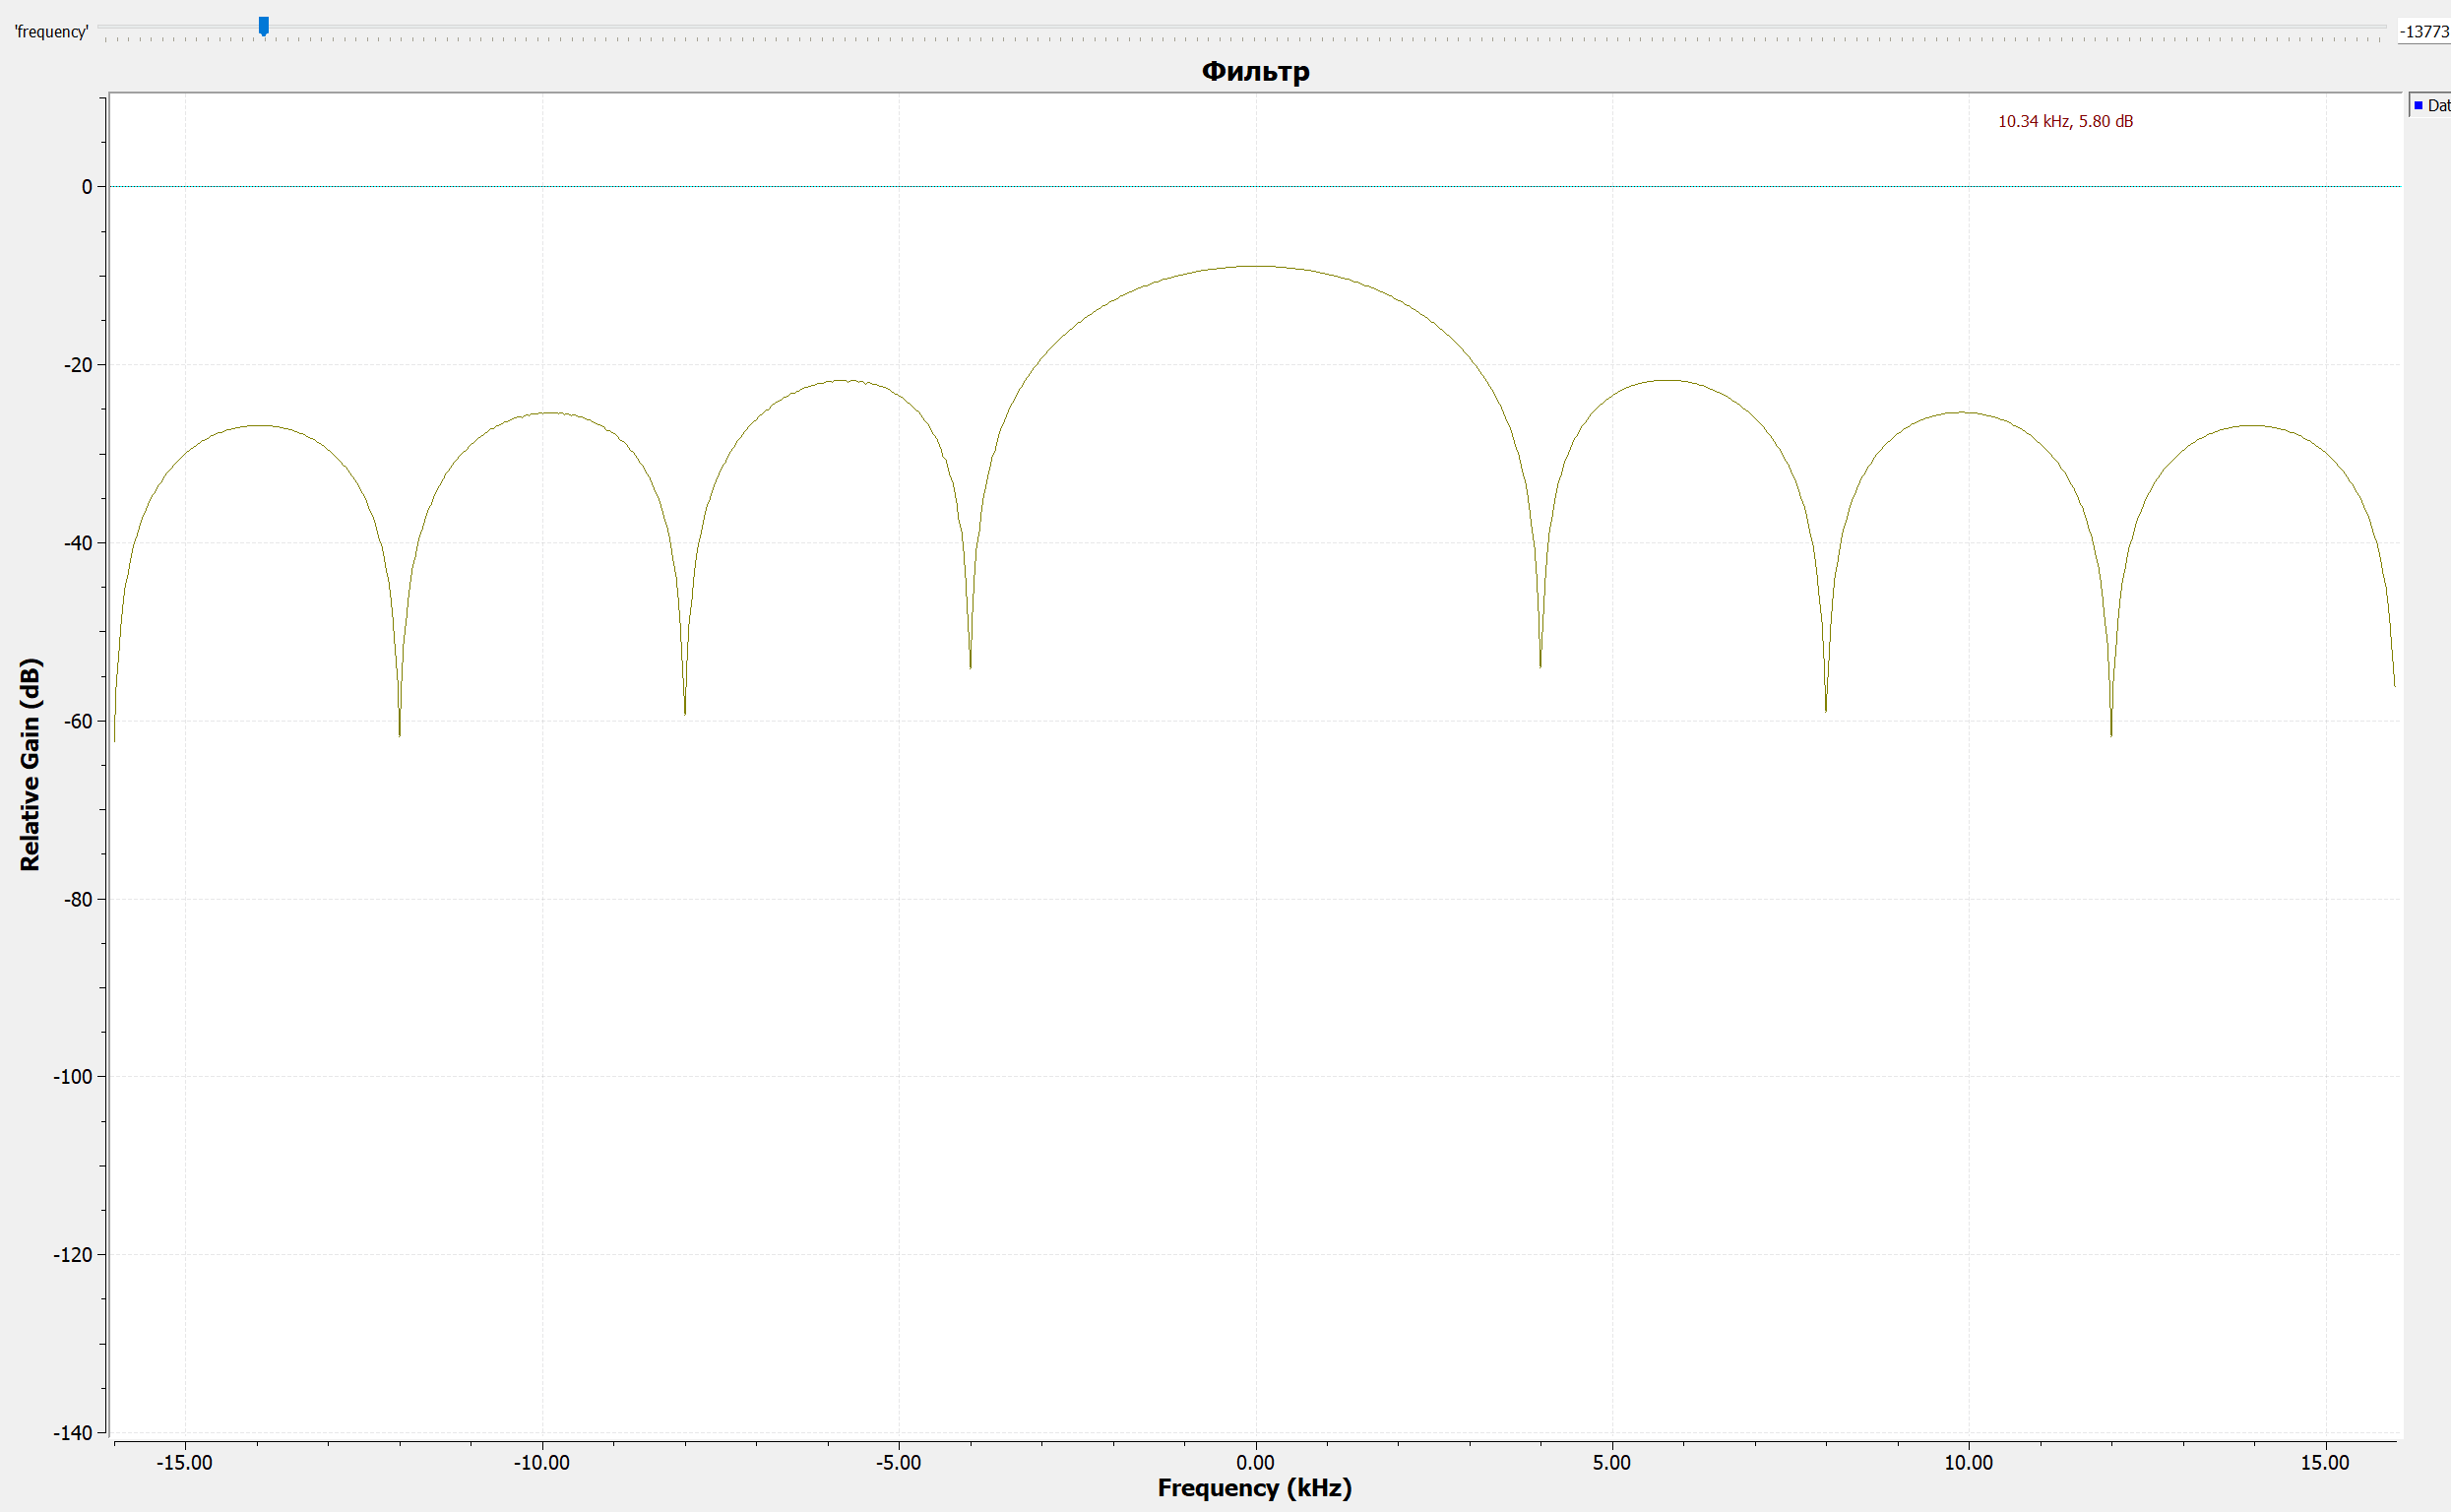
\includegraphics[width=.7\textwidth]{graph_2}
    \caption{График максимальных значений сигнала для 2 схемы.} %% подпись к рисунку
    \label{fig:graph_2} %% метка рисунка для ссылки на него
\end{figure}

\subsubsection{Анализ графика}

\hspace{1.15cm}Полученный график (Рис. \ref{fig:graph_2}) демонстрирует частотную характеристику 
фильтра после применения настройки Max Hold и изменения значения частоты от -16000 до 16000 Гц. 
Этот график показывает, как фильтр изменяет амплитуду сигнала на различных частотах в указанном 
диапазоне.

\begin{itemize}
    \item \textbf{Полоса пропускания:}
    Виден множественный узор пиков и провалов, что типично для фильтра с полосой пропускания, повторяющейся через определенные интервалы. Основные пики соответствуют частотам, которые фильтр пропускает, а глубокие провалы (нулевые точки) показывают частоты, на которых происходит значительное подавление сигнала.
    
    \item \textbf{Нулевые точки:}
    График показывает четко выраженные нулевые точки на определенных частотах, примерно каждые 5 кГц. Это указывает на то, что фильтр имеет структуру полосового подавления (notch фильтр) или эквалайзера с множественными полосами.
    
    \item \textbf{Поведение на краях диапазона:}
    На краях диапазона (-16 кГц и 16 кГц) фильтр также показывает определенное подавление, что соответствует ожиданиям для большинства FIR фильтров.
\end{itemize}

\paragraph{Поведение на разных частотах:}

\begin{itemize}
    \item \textbf{Центральная полоса (0 кГц):}
    Как видно из графика, около 0 кГц и на частотах около 5 кГц, 10 кГц и -5 кГц, -10 кГц фильтр пропускает сигнал с относительно меньшим подавлением (до -20 дБ).
    
    \item \textbf{Нулевые точки:}
    В интервалах около -15 кГц, -10 кГц, -5 кГц, 5 кГц, 10 кГц и 15 кГц сигнал подавлен на глубину до -60 дБ, что указывает на эффективное подавление этих частот фильтром.
    
    \item \textbf{Поведение в промежуточных точках:}
    На промежуточных частотах, между основными пиками и нулевыми точками, фильтр показывает умеренное подавление, что типично для частотных характеристик FIR фильтров.
\end{itemize}

\paragraph{Соответствие ожиданиям:}
График соответствует ожиданиям, демонстрирует ожидаемое поведение FIR фильтра с повторяющимися 
полосами подавления и пропускания. Эти результаты свидетельствуют о том, что фильтр успешно 
выполняет свою функцию по выборочному подавлению и пропусканию частот в заданном диапазоне. Провалы 
на графике указывают на частоты, которые фильтр эффективно подавляет, а пики показывают частоты, 
которые он пропускает.

\subsection{Real to Complex Filter}

\hspace{1.15cm}Многие блоки фильтрации имеют опции для выбора комбинаций вещественных или сложных 
типов данных для входных и выходных данных, а также вещественных или комплексных весов фильтров. 
В этом примере демонстрируется один из методов использования комплексных весовых коэффициентов 
фильтров для преобразования реального сигнала в комплексный.

\subsubsection{Изменение схемы}

\begin{itemize}
    \item Снова включим блок \textbf{Low-Pass Filter Taps} и удалим созданную в предыдущем 
    пункте переменную \textbf{boxcarFilter}.
    \item Отводы \textbf{lowPassTap} используются в качестве основы для комплексного полосового 
    фильтра. Создадим переменную \texttt{n} со значением \texttt{np.arange(0,len(lowPassTaps))}, 
    которая будет выдавать массив целых чисел от \texttt{0, 1, 2, 3, ...} до длины \textbf{lowPassTaps}.
    \item Также, создадим переменую \texttt{frequencyShift} со значением \texttt{np.exp(2j*np.pi*0.25*n)},
    которая представляет собой сложную синусоиду с частотой \(\frac{1}{4}\) частоты дискретизации. Переменная 
    \texttt{frequencyShift} изменяет центральную частоту lowPassTaps от 0 до \(\frac{1}{4}\) частоты дискретизации.
    \item Заменим элемент \textbf{lowPassTaps} на \textbf{bandPassTaps} в фильтре Frequency Xlating. 
    Отредактируем свойства источника сигнала и преобразуем его в реальный сигнал.
\end{itemize}

\vspace{0.2cm}После всех описанных ранее действий мы получим следующую схему:\\
\begin{figure}[H]
    \centering
    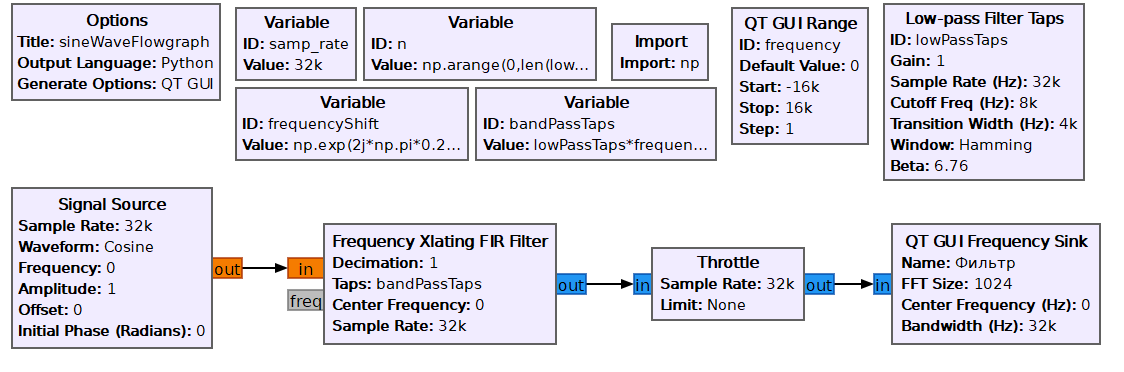
\includegraphics[width=.7\textwidth]{schem_3}
    \caption{Схема Real to Complex Filter.} %% подпись к рисунку
    \label{fig:schem_3} %% метка рисунка для ссылки на него
\end{figure}

\subsubsection{Анализ схемы}

Рассмотрим полученную выше схему (Рис. \ref{fig:schem_3}) подробнее.

\paragraph{Принцип работы}

\begin{itemize}
    \item Основной принцип схемы \texttt{"Real to Complex Filter"} заключается в разделении реального 
    сигнала на два компонента: вещественную и мнимую части. Это преобразование выполняется с 
    использованием фильтров сдвига и преобразования Гильберта, которые выделяют положительные и 
    отрицательные частоты.
\end{itemize}

\paragraph{*Преобразование Гильберта}

Преобразование Гильберта — это математическая операция, которая используется для создания аналитического сигнала из реального сигнала. Аналитический сигнал представляет собой комплексный сигнал, в котором вещественная часть является исходным сигналом, а мнимая часть — его преобразованием Гильберта.

\textbf{Определение}

Преобразование Гильберта \( \mathcal{H}(x(t)) \) для сигнала \( x(t) \) определяется следующим образом:

\[
\mathcal{H}(x(t)) = \frac{1}{\pi} \, \mathrm{P.V.} \int_{-\infty}^{\infty} \frac{x(\tau)}{t - \tau} \, d\tau
\]

где \(\mathrm{P.V.}\) обозначает главное значение интеграла.

В частотной области преобразование Гильберта можно записать как:

\[
\mathcal{H}(x(t)) = \mathcal{F}^{-1} \left\{ -j \cdot \mathrm{sgn}(f) \cdot \mathcal{F}\{x(t)\} \right\}
\]

где \( \mathcal{F} \) и \( \mathcal{F}^{-1} \) обозначают прямое и обратное преобразование Фурье, соответственно, а \(\mathrm{sgn}(f)\) — знаковая функция, определённая как:

\[
\mathrm{sgn}(f) = \left\{
\begin{array}{ll}
1, & \textnormal{если } f > 0 \\
0, & \textnormal{если } f = 0 \\
-1, & \textnormal{если } f < 0 
\end{array}
\right.
\]

\textbf{Аналитический сигнал}

Аналитический сигнал \( z(t) \) для реального сигнала \( x(t) \) формируется следующим образом:

\[
z(t) = x(t) + j \mathcal{H}(x(t))
\]

где \( j \) — мнимая единица.

\textbf{Свойства преобразования Гильберта}

\begin{itemize}
    \item \textbf{Изменение фазы:} Преобразование Гильберта сдвигает фазу сигнала на \( \pm 90^\circ \).
    \item \textbf{Частотная характеристика:} В частотной области преобразование Гильберта умножает спектр сигнала на \( -j \cdot \mathrm{sgn}(f) \).
    \item \textbf{Отделение положительных и отрицательных частот:} Преобразование Гильберта используется для создания аналитического сигнала, который содержит только положительные частоты.
\end{itemize}


\paragraph{Предположения о поведении сигнала}
На всем промежутке от -16 до 16 кГц выходной сигнал будет вести себя следующим образом:

\begin{itemize}
    \item \textbf{От -16 кГц до -8 кГц}: Эти частоты будут подвергнуты фильтрации и, скорее всего, их амплитуда будет значительно уменьшена. Это связано с тем, что фильтр предназначен для подавления этих частот.
    \item \textbf{От -8 кГц до 0 кГц}: В этом диапазоне сигналы будут преобразованы в комплексные, и их амплитуда останется на прежнем уровне, так как это диапазон частот, на который настроен фильтр.
    \item \textbf{От 0 кГц до 8 кГц}: Аналогично предыдущему диапазону, сигналы в этом интервале будут преобразованы в комплексные и сохранят свою амплитуду.
    \item \textbf{От 8 кГц до 16 кГц}: Эти частоты будут подавлены, и их амплитуда будет уменьшена фильтром.
\end{itemize}

\paragraph{Пояснения}

Основное предположение основано на принципе работы фильтров и преобразования Гильберта, которые 
используются для создания комплексного сигнала из реального. Они эффективно разделяют положительные 
и отрицательные частоты, позволяя сохранять информацию о фазе и амплитуде сигнала в интересующем 
диапазоне (от -8 кГц до 8 кГц) и подавляя ненужные частоты.

Таким образом, выходной сигнал будет состоять из комплексных значений в диапазоне от -8 кГц до 8 кГц с сохраненной амплитудой, тогда как сигналы за пределами этого диапазона будут значительно подавлены.

\subsubsection{Запуск блок-схемы}
\hspace{1.15cm}Проверим наши предположения, выполнив запуск схемы, представленной на Рис. 
\ref{fig:graph_3}. Установим настройку \textit{Max Hold} (Максимальное удержание). 
Когда эта опция включена, график показывает максимальное значение сигнала, которое было 
достигнуто в течение заданного времени, а затем удерживает его на экране. В результате получим 
график Комплексного фильтра с преобразованием реального сигнала:\\
\begin{figure}[H]
    \centering
    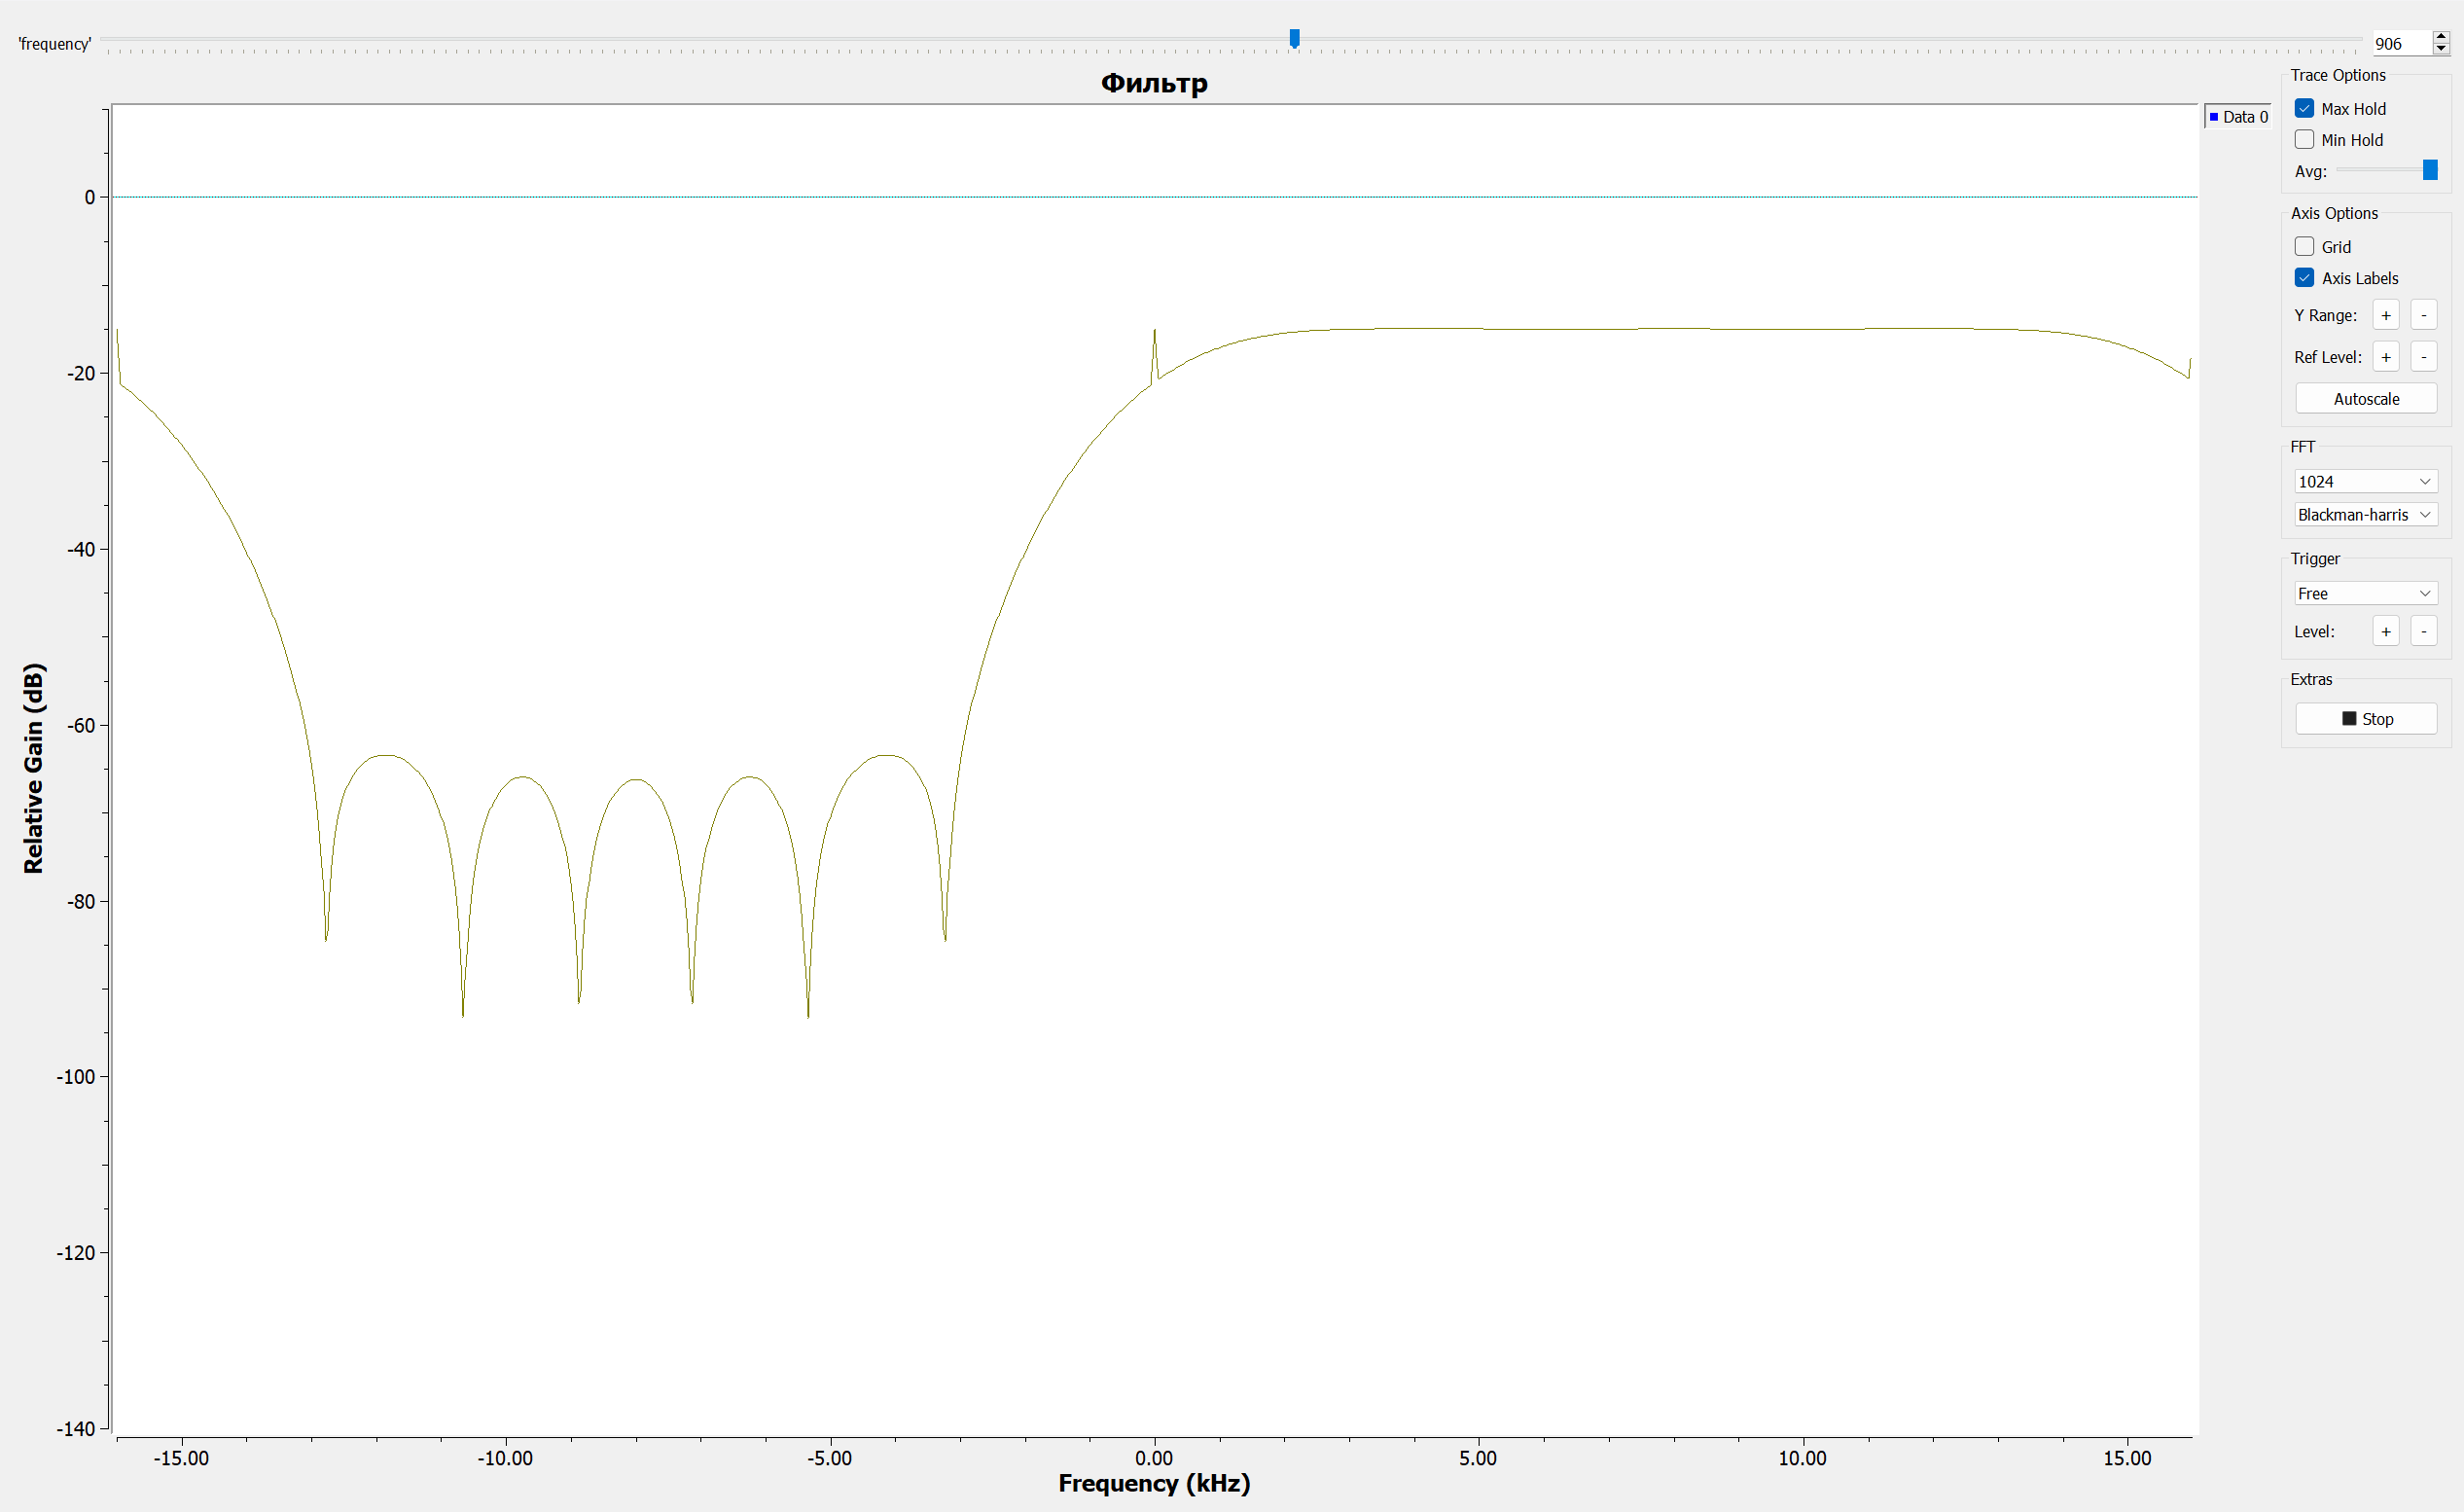
\includegraphics[width=.7\textwidth]{graph_3}
    \caption{График максимальных значений сигнала для 2 схемы.} %% подпись к рисунку
    \label{fig:graph_3} %% метка рисунка для ссылки на него
\end{figure}

\subsubsection{Анализ графика}

\hspace{1.15cm}Полученный график (Рис. \ref{fig:graph_3}) демонстрирует частотную характеристику 
фильтра после применения настройки Max Hold и изменения значения частоты от -16000 до 16000 Гц. 
Этот график показывает, как фильтр изменяет амплитуду сигнала на различных частотах в указанном 
диапазоне.

\begin{itemize}
    \item \textbf{Полоса пропускания:}
    Частоты в диапазоне от -8 кГц до 8 кГц соответствуют полосе пропускания нашего фильтра. В этой области амплитуда сигнала остается значимой, и мы можем наблюдать как реальную, так и мнимую части сигнала.
    
    \item \textbf{Нулевые точки:}
    От -16 кГц до -8 кГц и от 8 кГц до 16 кГц - это области, где фильтр подавляет сигнал. В этих диапазонах амплитуда сигнала близка к нулю, что соответствует нашим ожиданиям от фильтрации нежелательных частот.
    
    \item \textbf{Пик при 12 кГц:}
    Важно отметить, что мы наблюдаем пик амплитуды сигнала при 12 кГц, что также соответствует нашим предположениям о поведении сигнала в этой области. Этот пик свидетельствует о наличии сигнала с высокой амплитудой в указанном диапазоне частот.
\end{itemize}

\paragraph{Соответствие ожиданиям:}
Анализ графика подтверждает, что наблюдаемые результаты полностью соответствуют нашим ожиданиям. 
Полоса пропускания фильтра эффективно сохраняет амплитуду сигнала в заданном диапазоне частот, в 
то время как нежелательные частоты успешно подавляются. Пиковая амплитуда при 12 кГц, 
соответствующая нашему сигналу, подтверждает правильность выбора частоты и эффективность 
применяемых методов обработки сигнала.


\newpage
\section{Вывод}
\hspace{1.15cm}В ходе данной лабораторной работы мы изучили процесс проектирования фильтров в 
среде GNU Radio. Мы рассмотрели основные виды фильтров (низкочастотные, высокочастотные, полосовые 
и режекторные), методы их проектирования с использованием оконных функций и сглаживания, а также 
проанализировали амплитудно-частотные характеристики (АЧХ) разработанных фильтров. 

\hspace{1.15cm}Фильтры были реализованы в GNU Radio и проверены на реальных сигналах, что 
позволило оценить их эффективность и влияние на обрабатываемые сигналы. В результате работы мы 
пришли к следующим выводам: проектирование и анализ фильтров являются ключевыми задачами в 
цифровой обработке сигналов (DSP), а правильный выбор типа и параметров фильтра критически важен 
для таких задач, как удаление шумов и выделение полезного сигнала. 

\hspace{1.15cm}Полученные навыки работы с GNU Radio полезны для дальнейших исследований и 
профессиональной деятельности в телекоммуникациях, радиотехнике и цифровой обработке сигналов. 
Фильтры широко применяются в телекоммуникациях, медицине и аудиотехнике, улучшая качество сигналов 
и подавляя нежелательные шумы. Лабораторная работа углубила наши знания и предоставила ценные 
практические навыки.
\end{document}